\newpage
\section{Vererbung (Inheritance)}
	Vererbung ist ein Konzept, das es erlaubt, neue Klassen auf Basis von alten Klassen zu definieren. Die neuen (Unter-, Sub-) Klassen besitzen, ohne Eingriffe in den
	Sourcecode der bereits bestehenden (Ober-, Basis-, Super-) Klassen, all deren Eigenschaften, sie erben deren Verhalten und Daten. Den Vorgang der Vererbung nennt man auch Ableiten.\\
	\begin{minipage}[t]{7 cm}
		\subsection{Einsatz der Vererbung}
		\begin{compactitem}
			\item Bestehende Klassen erweitern (zus�tzliche Attribute und Elementfunktionen)
			\item Bestehende Methoden einer Basisklasse �ndern (�berschreiben)
			\item Einsatz nur wenn eine \textbf{IST-EIN} Beziehung besteht (z.B. Baum \textbf{ist eine} Pflanze, Blume \textbf{ist eine} Pflanze)\\
		\end{compactitem}
		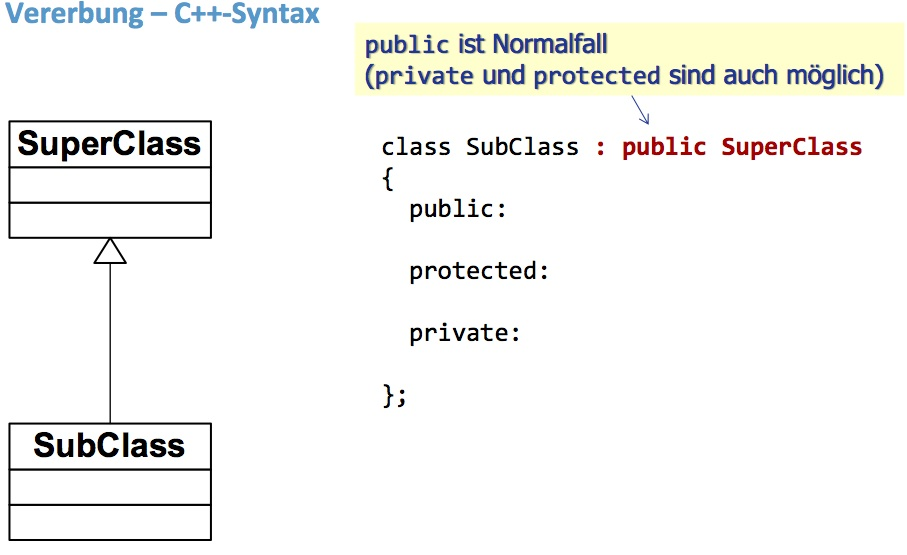
\includegraphics[width=1\textwidth]{pics/bsp_Vererbung.jpg}
		\subsection{Ableiten einer Klasse}
			Der Syntax der Ableitung einer Klasse ist oben aufgef�hrt. Als weiteres Beispiel ist im Anhang das Beispiel des \lc{ComicCharacters} und \lc{SuperHero} eingef�gt. \lc{SuperHero} \textbf{ist ein} \lc{ComicCharacter}.
			\begin{compactitem}
				\item \lc{friend}-Beziehungen werden nicht vererbt
				\item Ein Objekt einer Oberklasse kann Objekte einer beliebigen Unterklasse aufnehmen aber nicht umgekehrt (Substitutionsprinzip)
				\item Ein Objekt einer vererbten Klasse enth�lt alle Teile der Basisklasse und zus�tzlich noch die spezifischen eigenen Teile.
				\item Das Objekt ist somit mindestens so gross wie jenes der Basisklasse (es gibt keine Vererbung \lc{by reference})
				\linebreak
			\end{compactitem}
			\lstinputlisting[language=C++,tabsize=2]{code/substitutionsprinzip.cpp}
	\end{minipage}	
	\hspace*{0.5cm}
	\begin{minipage}[t]{11.5 cm}
	\subsection{Zugriff auf Elemente der Basisklasse}
		\textbf{Bei Vererbung mit \lc{public} (Normalfall):}
			\begin{compactitem}
				\item Zugriff m�glich auf alle \lc{public}- und \lc{protected}- Elemente der Basisklasse, die Zugriffsrechte 
				(\lc{public}, \lc{protected}) der Basisklasse werden in der abgeleiteten Klasse beibehalten
				\linebreak
			\end{compactitem}
		\textbf{Bei Vererbung mit \lc{protected}:}
			\begin{compactitem}
				\item Zugriff m�glich auf alle \lc{public}- und \lc{protected}- Elemente der Basisklasse, die Zugriffsrechte 
				von \lc{public} und \lc{protected} der Basisklasse werden in der abgeleiteten Klasse zu \lc{protected}
				\linebreak
			\end{compactitem}
		\textbf{Bei Vererbung mit \lc{private}:}
			\begin{compactitem}
				\item Zugriff m�glich auf alle \lc{public}- und \lc{protected}- Elemente der Basisklasse, die Zugriffsrechte von \lc{public} und \lc{protected} der Basisklasse werden in der abgeleiteten Klasse zu \lc{private}
				\linebreak
			\end{compactitem}
		\textbf{Bei allen drei: kein Zugriff auf \lc{private}-Elemente der Basisklasse}
		%\lstinputlisting[language=C++,tabsize=2]{code/privateFehler.cpp}
		\vspace*{0.3cm}
		\subsection{Slicing Problem}
			Links: Beim Kopieren werden nur die \lc{ComicCharacter}-Teile ber�cksichtigt. Durch das Kopieren wird alles �berfl�ssige 
			weggeschnitten, �brig bleibt ein reines \lc{ComicCharacter} Objekt im Fall von \lc{s} f�hrt dies dazu, dass die erweiterten \lc{SuperHero} Daten und Funktionen verloren gehen.\newline
			Rechts: Hier wird dank des Referenzparameters der gesamte Superheld ausgegeben.\newline
			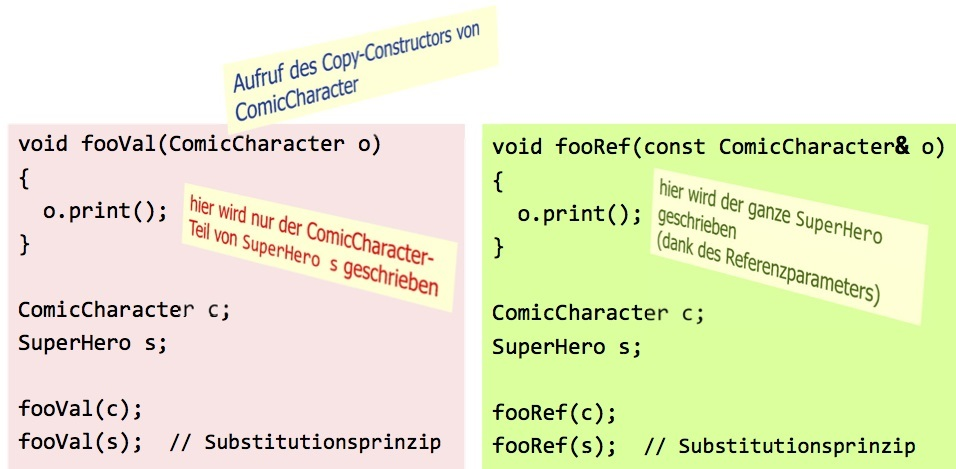
\includegraphics[width=1\textwidth]{pics/SlicingProblem.jpg}
		%\end{minipage}	
		\subsection{Vererbung und G�ltigkeitsbereiche}
			Die Klasse \lc{C} enth�lt alle Elemente von \lc{B} und somit auch von \lc{A}. \lc{A} jedoch hat kein \lc{i} und kann auch von keiner Oberklasse erben, dies ergibt den Fehler. \lc{B} hat zwar auch kein \lc{j}, erbt aber das von \lc{A}.\newline
			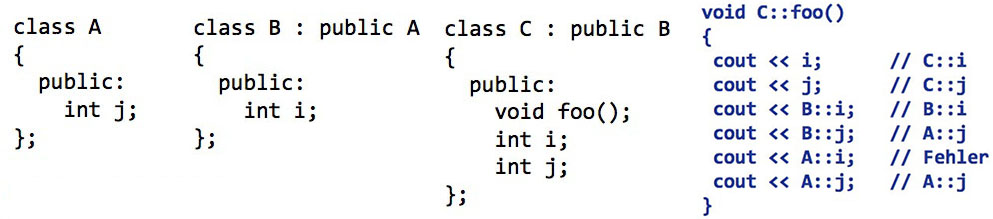
\includegraphics[width=1\textwidth]{pics/zugriffVererbung.jpg}
	\end{minipage}
	\subsection{Elementfunktionen bei abgeleiteten Klassen}
	\vspace*{-0.4cm}
	\begin{minipage}[t]{12 cm}
    	\subsubsection{Konstruktoren}
    		In einem Konstruktor m�ssen alle Elemente eines Objekts (auch die ererbten) initialisiert werden. Folgendes Beispiel zeigt die direkte Initialisierung aller Elemente. Vor allem bei grossen oder mehreren Klassen ist dies nicht zielf�hrend. Stattdessen wird das Chaining Prinzip angewandt. Falls kein Aufruf eines Basislklassen-Konstruktors in der Initialisierungsliste eines Konstruktors erscheint, so f�gt der Compiler automatisch den Default-Konstruktor der Basisklasse ein.
   			\lstinputlisting[language=C++,tabsize=2]{code/initVererbungKonstruktor.cpp}
   		\subsubsection{Initialisierung durch Chaining}
   			Jede Klasse erledigt nur die eigenen Aufgaben. Aufgaben, die ererbte Methoden �bernehmen k�nnen, werden diesen delegiert (Aufruf der jeweiligen Konstruktoren)\newline
   			\textbf{Wichtig: die Elemente der Basisklasse m�ssen immer als erste initialisiert werden}
    		\lstinputlisting[language=C++,tabsize=2]{code/initVererbungChaining.cpp}
	\end{minipage} \hspace*{0.5cm}
	\begin{minipage}[t]{6.5 cm}
		\subsubsection{Copy-Konstruktor}
			\begin{compactitem}
				\item Wenn kein Copy Constructor explizit definiert wird, so erzeugt das System einen
				\item Darin wird immer (ebenfalls automatisch) zuerst der Copy Constructor der Basisklasse aufgerufen
				\linebreak
			\end{compactitem}
		\subsubsection{Destruktor}
			\begin{compactitem}
				\item Auch Destruktoren werden nach dem Chaining-Prinzip aufgebaut
				\item Jede Klasse k�mmert sich um die eigenen Attribute und �berl�sst jene der
				Basisklasse auch der Basisklasse
				\item Destruktoren m�ssen nie explizit aufgerufen werden. Der Destruktor der
				Basisklasse wird \textbf{am Schluss} des Destruktors immer automatisch aufgerufen\newline
				Ein leerer Destruktor der Art
				\lstinputlisting[language=C++,tabsize=2]{code/destructor.cpp}
				ruft automatisch den Basisklassen-Destrukor (von \lc{ComicCharacter}) auf.
				\\
			\end{compactitem}
		\subsubsection{�berschreiben von ererbten Methoden}
			\begin{compactitem}
				\item Falls ererbte Methoden nicht das erf�llen, was eine bestimmte Klasse m�chte, dann
				k�nnen diese Methoden neu definiert (�berschrieben) werden.
				\item Methoden, welche in einer abgeleiteten Klasse �berschrieben werden k�nnen, m�ssen in der Basisklasse mit \lc{virtual} gekennzeichnet sein.
				\item Ab \lc{C++11} sollen in der Unterklasse die �berschriebenen Methoden mit \lc{override} gekennzeichnet werden. Damit weiss der Compiler, dass mit dieser Methode eine andere �berschrieben wird.
				\item Im Anhang wird dieses �berschreiben einer Methode beim \lc{SuperHero} f�r die Funktion \lc{dance()} vorgenommen. W�hrend ein normaler \lc{ComicCharacter} tanzt, wird diese Funktion beim \lc{SuperHero} �berschrieben und mit tanzt nicht �berschrieben.
				\linebreak
			\end{compactitem}		
	\end{minipage}   